\documentclass[a4paper,11pt]{article}
\usepackage[margin=3cm]{geometry}
\usepackage{float}
\usepackage[T1]{fontenc}
\usepackage[utf8]{inputenc}
\usepackage{amsfonts}
\usepackage{graphicx}
\usepackage{bm}
\usepackage{varioref}
\usepackage[english]{babel}
\usepackage{hyperref}
\usepackage{tikz}
\usetikzlibrary{arrows,decorations.pathmorphing,backgrounds,positioning,fit,petri}
\usepackage{enumitem}
\usepackage{newclude}
\newcommand{\field} [1] {\mathbb{#1}}
\newcommand{\mil}{Musik i Lejet }
\newcommand{\milNO}{Musik i Lejet}
\begin{document}

\begin{titlepage}
\centering \parindent=0pt
\newcommand{\HRule}{\rule{\textwidth}{1mm}}
\vspace*{\stretch{1}} \HRule\\[1cm]\Huge\bfseries
MIL Project\\\emph{Musik i Lejet}\\[0.7cm]
\HRule\\[4cm]  \large  Jägerne
\\Jacob Stenum Czepluch (jstc@itu.dk), \\

\vspace*{\stretch{2}} \normalsize %
\thispagestyle{empty}
\begin{flushleft}
BFOP \\
Bachelor in Software Development\\
IT-University of Copenhagen\\
December 15, 2013 \end{flushleft}
\end{titlepage}

\tableofcontents
\pagebreak

\pagebreak
\section{LOL}
pops


%!TEX root = /Users/Abj/git/MiL/report/report.tex
\part{Summary}

\section{About}
Introduction... 

How can the board delegate responsibility of the planning and execution of Musik i Lejet to the management? 

Measurements:
Topics on board meeting minutes, identified by the board as topics subject to management, should be reduced by x%


\section{List of activities}
We have created a list to give an overview over which kind of activities we have conducted doing the project and when we did them. The list can be found in appendix XX
\begin{center}
\begin{table}
    \begin{tabular}{|p{3cm}|p{3cm}|p{3cm}|p{6cm}|}
    \hline
    Date & Type of activity & Participants & Comments \\
    29 - 09 - 13 & (non-formal?) Interview & MiL: Andreas Workgroup: All & The workgroup presented the scope(?) of the course and got an initial idea of the organization and the role that Andreas have in MiL.  \\
    31 - 10 - 13 & (formal?) interview  & MiL: Christian og Stakkeman &  .......  \\
    \end{tabular}
\end{table}
\end{center}
\section{Figure of organization}
First draft of organizational diagram. Needs to be confirmed by MiL
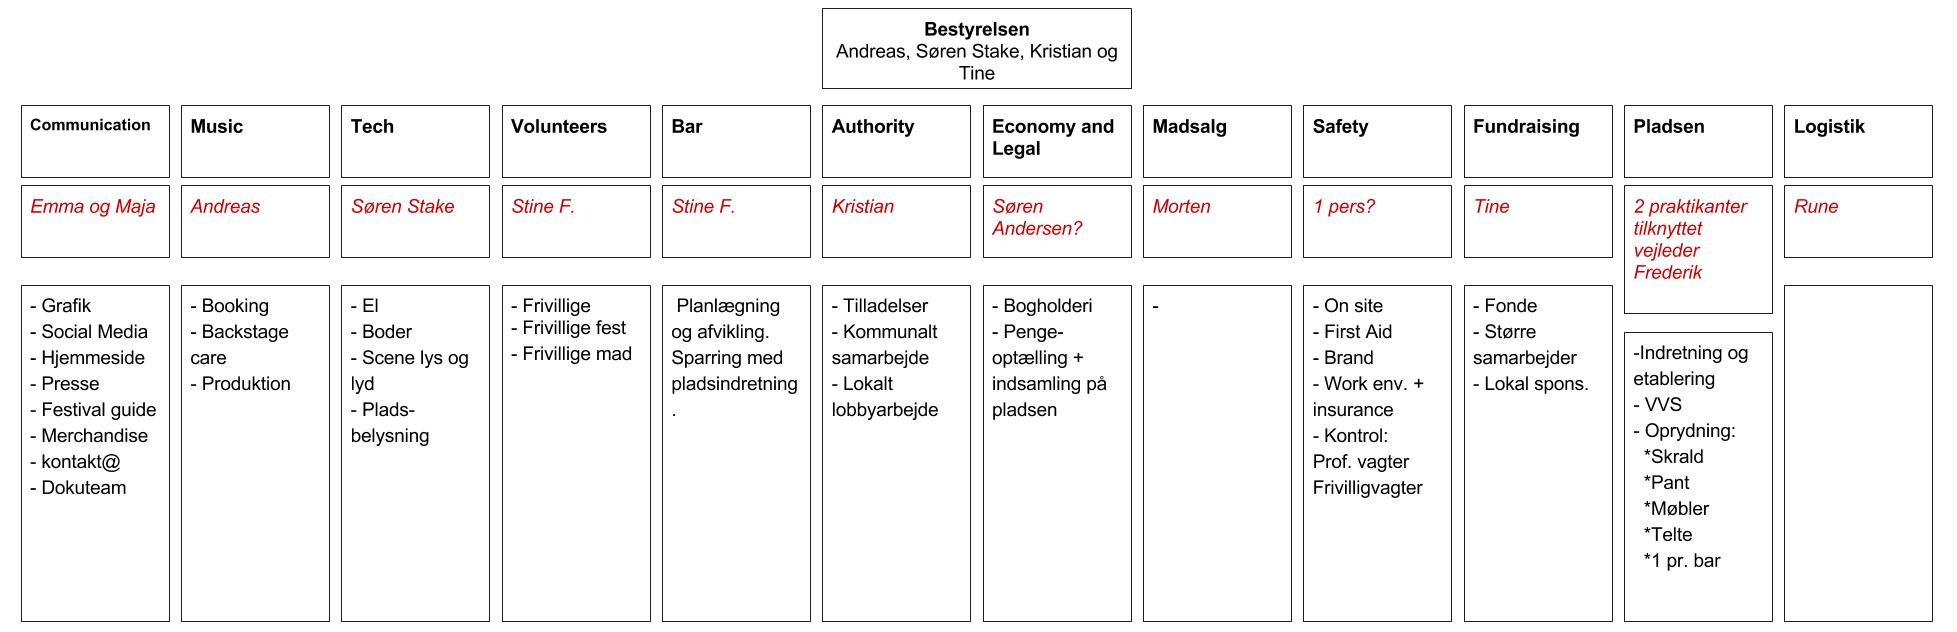
\includegraphics[scale=0.3, angle=90]{Pictures/MIL_Organisational_chart-Ledelsen.jpg}
\section{Business and IT scope}
For this project the workgroup have chosen to focus on the managing part and more specific the board of Musik I lejet. We will also look at how the internal communication is shared between all members and what kind of work processes is in play when planning the festival. \\
Must of the communication is done at Musik i Lejet's Podio site and therefore we will direct our attention and observations towards that platform. Since this projects is done before the actual festival takes place, we will primarily focus on IT used before the festival, which to our belief, is only Podio.  

\part{In-line Analysis}

\section{Business Strategy}
The main objective of Musik i Lejet is to provide a cultural offer in the local community of Tisvildeleje, both as an offer to the local populous, and also to attract business to the community. This is achieved by a non-profit, cost driven business model, that relies heavily on volunteer work, grant money and private sponsorship. Cultural and economic value is generated by offering musical entertainment for a variety of customer segments, such as music enthusiasts, families with children and customers interested in attending parties.
\\ \\
Keeping a well defined and contemporary musical profile is essential for Musik i Lejet to fulfill both its cultural objectives, and to make the festival competitive with other festivals of the same size, addressing the same customer segments. Moreover, diversity within the festivals audience is of huge importance to Musik i Lejet. This is in part achieved by offering a wide selection of music in many different genres, but also by keeping ticket prices low, and providing free admission for children and the elderly.
\\ \\
The main challenges for Musik i Lejet include maintaining relationships with and interest from sponsors and cultural foundations, securing the necessary number of volunteer workers, coordinating the efforts of the 20-30 people who, without a physical and centralized work space, arrange the festival in their spare time, and obtaining contracts with contemporary and popular performing artists to an affordable price.

\section{Environment}
When studying MiL it is of importance to view it in the relative perspective of its surroundings to be able to determine strengths/weaknesses as well as relations, ultimately to support potential solutions. In this case we deal with the remaining forces of danish music festivals.
\\  \\
The industry of danish music festivals is a healthy and growing market showing indications of trends towards an increasing appreciation of larger live events. Many festivals exists as of today, but differentiate significantly in vision, identity, and size. This means that when considering the market, competition to MiL can not be inferred if they do not target the same customer segments. Due to MiLs price and target segments, opposing threats are few in numbers, e.g. Wonderfestiwall and trailerpark festival. This compitition fails to compete with MiL by due to the significent difference in ticket price.
\\  \\
Stable relationships with providers and stakeholders are of big part of what makes MiL possible, and are therefore an important aspect to maintain and care. Due to success throughout MiLs past years of events can provide stability as an organisation through factors such as: sold out events, positive publicity and continous increase in revenue. With this MiL has established quality cooperation agreements providing security and avoiding risk at depencies.
\\  \\
A potential risk occuring as a product of MiLs increasing success is the organisations capability of scaling its internal resources to match a larger event while maintaining the same value offer - This in view of the environment MiL lacks experience due to its relative young age. Failing to being able to cope with expansion could result in increased ticket prices. This would remove MiLs advantage, enabling competition to become competition


\section{Work Domains}
\label{sec:work_domains}
\subsection{The board}
\label{sub:the_board}
The main responsibility of the board is to make all major decisions regarding the execution of the
festival. They are also responsible for all strategic decisions and they handle the booking of
some of the big artists and the approval of expensive contracts and deals that the teams make.

\subsection{The team leaders}
\label{sub:team_leaders}
The team leaders each have an area of responsibility which results in a team leader being
responsible and the leader of a team of volunteers that focus on a specific area of the festival
planning. As seen in the \ref{sub:organisation} there are 12 independent teams. The most important
role of a team leader is to communicate with the other team leaders and give feed back to the board
regarding the status of the team's current tasks. Team leaders meeting are held once every ?????,
where the team leaders give status updates to each other and discuss inter team problems and
deadlines.

\subsection{The team members}
\label{sub:team_members}
A team member is simply a volunteer that help out with the planning of the festival, and not only
the execution. As a member of a team you will be given different tasks accomplish depending on which
team you are in. If you are in the bar team, a task could be to make sure that offers for bar tents
have been obtained before a certain deadline. 


%!TEX root = /Users/Abj/git/MiL/report/report.tex
\part{In-depth Analysis}

\section{Organizational setup, key players and KPI's}
\subsection{Organizational setup}
\subsubsection{Structural Change}
Before the project period was started the organization initiated a structural change. This influenced the board, but mostly the planning group, since this was expanded from X to Y members. This change was conducted in order to move and spread the knowledge and responsibility from the board across the organization, by delegating responsibility to leaders in different planning teams(interview kilde).

\subsection{Key Players}
Several types of key players can be identified in the organisation. Before the structural change, the level of key player, was determined by each persons experience with planning of Mil. Naturally, most of the key players was also part of the board.\\
With the newly structural change, these players are made responsible for a team, which enforces two things. Firstly, a lot of the planning are moved away from the board. Second, when delegating a person as a leader for a team, the knowledge for this particular area of planning is more assigned to a role in a team instead of a specific person. The consequences of this change, is that more key players can be identified, which creates more dependencies between the different area of planning, since more people are involved(kilde på at flere mennesker skaber mere afhængigheder).\\
Thereby, the current most interest key players are the leaders of each teams, which the stakeholder analysis in appendix xx suppports.\\
Bilag: STAKEHOLDER ANALYSIS??????\\

\subsection{Key Performance Indicators}
Top level KPI -> deadlines eksempel\\

Bilag:\\
Top level KPI's\\
finanical Stability\\
	- Ticket price\\
	- keeping budget\\
Podio\\
- 24 hour rule\\

KPI's: Ticket price, financial stability, keeping the budgets, 24 hour rule of podio\\

At this point of the project we identified a number of KPI's and we will use this section to underline some of the aspects according to these.\\
As described in appendix xx MiL has several top level KPI's which is crucial in respect to customer satisfaction and the overall sale during the festival(kilde?). 

\section{Current work practices}
This section will describe some of the work there is, when working in the planning group of Mil. Before going in to the actual descriptions, we do however need to mention, that observing work practices in an organization as this, is not a trivial task. We have observed the work practices in the form of interviews and an observation at the General Assembly, which hardly can be formulated as actual practices, but more as a mean to work. However, we have found several things, which we believe can be used as documentation for the practices. \\
At the General Assembly a suggestion from the board was raised, about all members being charged a fee for being part of MiL. The board explained that this was more a matter of regulation of a union, and to get some financial advantages, than a need for payment. The non-board(?) members raised some concerns regarding this issue, as stated in appendix xx. Surprisingly, even though the non-board members raised strongly concerns, the board decided to proceed with the suggestion, without a voting about it. \\
The board also included a short presentation of Podio at the General Assembly. As stated in appendix xx the board wants to have all internal communication in the planning group at Podio. This was clearly a new tool for some of the leaders, which was stated in the form of different questions(kilde?). Most of the presentation was about the different subpages at Podio and how to create things like events and tasks. This gave some insight what Podio is cable of, but no introduction was given about when a task was done nor when a task should be created for another member (better examples?).\\

During the interview with Stine F the project group made her participate in a 'process'-game. Here the interviewers asked her to explain the task of booking volunteers for the festival. The result of this game can be seen in appendix xx. In our opinion it clearly shows that a lot can be done in termns of deadlines for bookings of volunteers and also the way its done.

- Stemning og struktur på General Forsamling (blandt andet forslag om kontigent blev ikke besluttet)\\
- Podio (manglende af done og done-done) og noget andet?\\
- Problem med høj overpris af hegn\\
- Beskrivelse af process spil

\subsection{Goals, problems, and needs}
In this section we will summarize the goals, problems, and needs that the
in-depth phase analysis has lead us to.

\subsubsection{Goals}
It is clear to us, according to \ref{interview source} that it is a goal for \mil to cut down
the amount of missed deadlines.
\\
Some parts of the board \ref{Kristian source} sees it as a goal that the
budget is not only kept, but that the offers collected on expensive things, are
also the best offers.
\\
There is also a certain desire \ref{Learn podio reference} that everyone knows
how to use Podio, since the board demands that Podio is the single point of
communication for \mil.

\subsubsection{Problems}
According to our analysis \ref{source}, some problems are made clear. \\
              \begin{itemize}
    \item It is neither clearly stated when different tasks are due to
    internally in the different groups nor between the working groups.
    \item People leaves out some information on Podio, because they do not know
    how to add it properly.
    \item There is no single place on Podio where all important deadlines are
    put.
    \item There is no clear guidelines for when a task is done.
    \item (Add more if any...)
\end{itemize}

\subsubsection{Needs}
After several interviews with different people from \mil, it is clear to us that
there are some common needs.
\begin{itemize}
    \item According to \ref{source} there is a need for a system that makes it
    clear to everyone which deadlines are due to when.
    \item Guidelines describing when a task is done are also needed
    \ref{source}.
    \item A common understanding and knowledge of how the basics of how Podio
    works, assuring that everyone is able to document the progress of their work
    and tasks is also needed \ref{source}.
\end{itemize}


\subsection{Ideas for solutions}
In this section we will discuss some of the ideas we have for technical
solutions to help ease the organisational restructuring of \mil.

\subsubsection{Podio workshop}
It has come to our attention when attending \ref{General Assembly Appendix} that
a lot of the volunteers have very little knowledge of how Podio works. Due to
this, one of our suggestions is to make a Podio workshop that teaches the basics
of Podio the way the board of \mil has in mind that is should be used.

\subsubsection{Podio tutorial}
In addition to this, a tutorial made in Podio that uses the features of Podio to
teach how Podio works, is also a solution that we believe to be very useful
\ref{reference to something about how good learning hands on is} in the process
of learning how to use Podio.

\subsubsection{Podio App}
Since it is a goal \ref{source to this} that all communication should take place
on Podio, we would like to make a Podio app that allows the user to make tasks
and dependencies for each area of responsibility in the different groups.

\subsubsection{Done and done done}
There is a concern amongst some of the board members \ref{source from meeting
with Andreas} that since each responsibility group now have their own budget to
administer they will not necessarily use energy to find the best offers on the
market. Our solution proposition is to make a rule that when a person gets the
responsibility to find offers on eg the fence surrounding the festival area, the
person has to collect three offers and the rest of the responsibility group now
has to decide which one is best. The task to find an offer on the fence is now
done, but it is not marked as done done before the contract is signed.

\subsubsection{Wiki}
We have also found out that it is a pain \ref{source to interview} to have a
common place to share knowledge between the groups. A possible solution to this
is to make an app that makes it really easy to add knowledge to a shared wiki
through Podio.


%!TEX root = /Users/Abj/git/MiL/report/report.tex
\part{Innovation}
%As the previous sections of the \texttt{In-depth phase} in part \ref{prt:in_depth_analysis},
%especially in section \ref{sub:goprne}, has shown,
%the organisation has room for optimisation and improvements. Based on the \ref{sub:ideas} that we
%have developed and the fact that the organisation wants to continue using Podio, we have chosen two that we believe will bring the most benefits to the organisation.
%We will in the following analyse both the solutions, and try to determine which will be the best or
%if a third solution will emerge from this analysis. A short description of the ideas in focus
%follows:


%1. Work processes for Podio\\
%In the previous the Diagnostic Map in section xx revealed several problem and related causes found in the organization. In 5b its said that the cause of this problem, is that their is too much off topic discussion and also that no real difference between pure informational topics and topics for discussions are in place within the organizational use of Podio. As Stine F also points out in 1a, the organization faces a problem about sharing of knowledge, since this is not documented properly on Podio.\\

%This solution proposal will attempt to structure work processes when using Podio and make guidelines for the information posted at Podio. This proposal will therefore be  directed at the use of Podio, with respect to the mentioned things in the above, and will keep to the organizations strategy about using Podio as their primary IT solution. 

%2. Podio App
%This solution consists of the development of a Podio application \footnote{https://developers.podio.com/doc/app-store}.
%The application will be used to create, store, and visualise tasks in- and externally in the teams.
%Thus, hopefully, making it very transparent which tasks are due to when.\\

\section{WORK PROCESSES}
\subsection{Visions for change}
The visions for this solution proposal is a bit different, than what is normally suggested as a
solution, since this does not contain an actual implementation of a new IT solution, but rather a
change in the way the current system is used by the organisation.
Podio is very customisable and offers per default the possibility to create your own applications
suited for your needs. This solution will however focus solely on changing the way the organisation
is using their current available tools and work practices in Podio.


%The overall vision for the change, can be divided in to these subsections:
\subsubsection{Information at Podio}
As mentioned earlier, and seen on Podio, a lot information is non-relevant for the actual planning and should therefore be elsewhere. Based on the analysis, we believe that the reason for this non-relevant information is on Podio is due to the relaxed working environment shared by the members and also the lack of formal guidelines for what kind of information should be posted on Podio, by whom and when.\\ 
We suggest that the board makes a formal description of these, by categorizing them after importance.
This will impact every member of the planning group and board, since an equal amount of non-relevant information seems to be posted between all members. \\

Make scenario for how this new work practice will be for the persons impacted by it(p191)
  
\subsubsection{Sharing of knowledge}
With an organization structured and based highly upon volunteers like Musik I Lejet, there is always a risk of people leaving the organization with short notice and taking valuable information and knowledge with them. Since this risk is hard to limit, the solution proposal will try to embrace the knowledge that the members poses and expose this at relevant places on Podio, for others to use. The challenge with this, is to find the persons holding the knowledge and exploring it, since some of it may be tacit(use different levels of knowledge theory). A challenge is also to document this is a right way, so it can be reused at a later point and saving in a place on Podio where others will be able to find it.\\
The team leaders is probably the target for this part of the solution, since most of these a highly experienced and has a good feel about the different areas of the organization.\\

Make scenario for how this new work practice will be for the persons impacted by it(p191)

\subsubsection{Sharing of decisions and agreements}
Throughout the analysis phase, it has been pointed out that members of the organization find it hard to find out what decisions and agreements there have been made and where it is documented. Reasons for this is the causes mentioned in 2b and 4b in the Diagnostic Map in appendix xx. MORE STUFF HERE\\ 
Make scenario for how this new work practice will be for the persons impacted by it(p191)

\subsection{Technology}
Since this solution is based on the IT system that the organisation already uses, there is no point
in explaining the technology too much. A short summary of Podio can be found in the glossary in
section \ref{sec:glossary} and \ref{sec:technology}.

\subsection{Work organization}
As mentioned above, this solution, does not need an implementation of a new IT system. It does how
ever consist of changes to the work organisations of the organisation. 
We have concluded in section \ref{podio bloat source} that a lot of the information and
communication on Podio is irrelevant to the planning of the festival. It seems that a good solution
to this, would be to make some guidelines in cooperation with the board that states what kind of
communication should take place on Podio and where it should take place. If most of the irrelevant
comments and posts dissapeared, the change of overlooking important information and deadlines
decreases. 
* Frivillig organisation, de gør det også for at have det sjovt
* 

\subsection{Qualification needs}

\subsection{Advantages and disadvantages}

\subsection{Finances}

\subsubsection{Roll out}

\subsubsection{Training}
Forslag: Experts and normal users
\subsubsection{Data conversion}
Converting all the existing Podio data to be alligned with the new formal structure for information, knowledge and decisions...

\subsection{Implementation strategy}
The must effective way this solution can be implemented in the organization will be as a pilot project, where selected members of the organization will be trained in how to use the formal ... 



\section{Podio extension}
\subsection{Visions for change}
\label{visions_for_change}
This solution is at its heart an interactive visualization of tasks and task dependencies across arranger teams. Tasks are communicated between arranger teams with the already present infrastructure present in Podio. The task window however, is extended with the following functionality and data:
\begin{itemize}
    \item Tasks can include subtasks. Subtasks are added to a task by pressing the "Add Subtask" button. When teams assign tasks to other teams, the receiving team may choose to define subtasks, that need to be completed before the assigned task can be completed. Subtasks can either be already existing tasks, or new tasks.
    \item Tasks include a "Done" description, in which the sender of the task may include a short description of when the task is considered to be done.
    \item Tasks are done when the receiving team presses the "Done" button under a task.
\end{itemize}
The data and functionality described above makes it possible to create a task map. The task map displays all active tasks in the system. A task is active if any of its subtasks are incomplete, or if it is itself a subtask to a task that is incomplete. Tasks are displayed graphically, with dependencies between them drawn as an directed arrow between them. Clicking a task will take the user to the task on Podio, where a detailed view of the task can be found. 
\\ \\
This solution will give arrangers an overview of deadlines, tasks associated with deadlines and dependencies between them across arranger teams, as to address problems discussed in (ref diagnostic map). By extracting deadline information and placing it collectively in the task map, confusion about where to find information about deadlines is reduced.


\subsection{Technology}
\label{sub:technology}
The solution uses the built in functionality of Podio to build custom Podio apps to create the needed modifications to Podio tasks. The task map is drawn on a webpage outside of the Podio domain, using the Podio REST API.

\subsubsection{IT systems and IT platform}
The solution is primarily dependent on the existing Podio platform. It is necessary that Podio maintains the possibility of defining custom apps and accessing Podio data through the REST API.

\subsubsection{User interfaces}
On Podio, the interface is built using the existing Podio app builder tools. The task map is displayed by some Web UI technology. Tasks are shown as nodes, and dependencies between them are shown as directed arrows. Task completion status is indicated graphically by color. (ref til mock up)

\subsection{Work organisation}
\label{sub:work_organisation}
Arrangers and team leaders will have to change their work-flow with creating tasks, to comply with the format described in section \ref{visions_for_change}. An introduction to using the task map must also be created. Some teams already use tasks (ref til podio analyse), and others do not. The teams that are not familiar with tasks will have to be introduced to them, and some encouragement and reinforcement is likely to be necessary.

\subsection{Qualification needs}
\label{sub:qualification_needs}
The solution depends on arrangers and team leaders using Podio correctly. This means that arrangers and team leaders must know how to use Podio.

\subsection{Advantages and disadvantages}
\label{sec:advantages_disadvantages}
\begin{center}
    \begin{tabular}{ | p{7cm} | p{7cm} |}
    \hline
    \textbf{Advantages} & \textbf{Disadvantages}  \\ \hline
     Raises awareness of deadlines and dependencies between teams & Risk of arrangers not using the system\\ \hline
     Makes information about deadlines easier to find & Time must be invested in teaching arrangers how to and when to create tasks\\ \hline
     Integrated with a system that is already known and used by arrangers and team leaders & Solution is dependent on Podio maintaining custom app possibilities and a Web service interface \\ \hline
    \hline
    \end{tabular}
\end{center}


\subsection{Finances}

\subsection{Implementation strategy}
The pilot project strategy is recommended for this solution. Potential short comings and problems can be corrected before trying it with the whole organization. The bar team, fetival site team and volunteer team are good candidates for pilot teams, as significant dependencies exist between them (ref til stine interview eller flowchart).

A possible challege when implementing the strategy is motivating arrangers and team leaders to assign tasks on Podio, instead of sending messages or posting on walls of other groups etc. One strategy is to demonstrate the value of the task map, and how the usefulness of this tool is increased for everyone, when more arrangers use the task feature of podio.


\appendix
\part{Appendix}
\section{Business Model} % (fold)
\label{sec:business_model}
\subsection{Customer Segments} % (fold)
\label{sub:customer_segments}
\begin{itemize}
	\item \textbf{Music enthusiasts}\\
			This customer segment is interested in experiencing live music, and discovering new artists. \ref{i2q2} \ref{i2q4}
	\item \textbf{Families with children}\\
			This customer segment wants cultural offers which include activities for the entire family, including children. \ref{i2q2}
	\item \textbf{Local populous}\\
			This customer segment is interested in strengthening the local community, for example through cultural events. \ref{i2q6}
	\item \textbf{Party people}\\
			These customers want to party. They are interested in affordable prices on alcohol, and offers of specific genres of party music. \ref{i2q5}
	\item \textbf{Sponsors}\\
			This segment is interested in branding itself as supporting both local cultural events, and danish music culture. \ref{i1q7}
	\item \textbf{Service providers}\\
		This segment is interested in using the festival as a platform for offering their goods and services to the audience of the festival. For example, this could be caterers interested in selling food at the festival \ref{i1q6}
\end{itemize}
\subsection{Value Propositions} % (fold)
\label{sub:value_propositions}
\begin{itemize}
	\item \textbf{Strong musical profile}\\
	 Musik i Lejet strives to maintain a well-defined and contemporary musical profile. This allows music enthusiasts to experience both popular artists and discover new music. \ref{i2q1} \ref{i2q2}
	\item \textbf{Free entrance for children and elderly}\\
	Entrance to the festival is free for children and the elderly. This makes the prospect of making the festival a family event more affordable. \ref{i2q2}
	\item \textbf{Designated children's stage}\\
	Each day, a number of artists performing children's music at a designated stage. This as desirable for families with children, as it makes the festival an event for the entire family. \ref{i2q2}
	\item \textbf{Nightly after-party}\\
	Each night an after-party is held on the beach, with DJs and an open bar. This is desirable to anyone interested in attending wild parties. \ref{i2q5}
	\item \textbf{Unique location}\\
	Musik i Lejet is held at the beach of Tisvildeleje. This adds to a unique festival atmosphere, and contributes to a strong brand for Musik i Lejet. This is valuable for anyone wanting to associate with the festival, and use the festivals image to brand themselves. Its also of interest to most of the customers who attend for the festival experience. \ref{i2q7}
	\item \textbf{History of sold out tickets}\\
	The festival is increasingly popular, and boasts a history of sold out tickets. This is assures sponsors of getting the desired exposure by supporting the festival with cash donations or goods and services. In addition, its attractive to service providers interested in selling services at the festival. \ref{i1q3}
	\item \textbf{Frequent coverage in media}\\
	Musik i Lejet is often mentioned in music and mainstream media. This is useful for sponsors, as a strong brand for festival reflects well on their involvement with it. \footnote{http://gaffa.dk/nyhed/78769} \footnote{http://politiken.dk/ibyen/nyheder/musik/ECE2005317/sommerferie-festival-samler-staerke-danske-navne-paa-stranden/}
	\footnote{http://soundvenue.com/musik/2013/02/musik-i-lejet-spiller-med-musklerne-46513}
\end{itemize}
\subsection{Channels} % (fold)
\label{sub:channels}
\begin{itemize}
	\item \textbf{musikilejet.dk}\\
		The festival uses the page musikilejet.dk, to provide information about the festival program, ticket sales (by a link to billetto.dk), and general information about the festival. The page also provides contact information on board members and arrangers in order for customers to be able to contact the relevant people int the organization.
		\footnote{http://musikilejet.dk/}
	\item \textbf{Local advertisement}\\
		Local advertisement is used to raise awareness of Musik i Lejet's services. Posters and brochures available at local businesses display information about the festival program and dates. \ref{i2q6}
	\item \textbf{Music media}\\
		Musik i Lejet offers accreditation to critics and journalists who visit the festival with the purpose of reporting on concerts and events. This means Musik i Lejet is often covered in magazines and newspapes such as Gaffa, Soundvenue, Politiken ect. \footnote{http://gaffa.dk/nyhed/78769}  \footnote{http://politiken.dk/ibyen/nyheder/musik/ECE2005317/sommerferie-festival-samler-staerke-danske-navne-paa-stranden/}
		\footnote{http://soundvenue.com/musik/2013/02/musik-i-lejet-spiller-med-musklerne-46513}
	\item \textbf{Social Media}\\
		Musik i Lejet extensively uses social media to promote the festival, in addition to receiving feedback from and communicating with customers. \footnote{https://www.facebook.com/musikilejet}
	\item \textbf{Billetto.dk}\\
		Musik i Lejet offers tickets in advance sale through billetto.dk \footnote{http://billetto.dk/musikilejet}
	\item \textbf{The festival site}\\
		The festival site is where all events and services are offered to customers. Tickets not sold in advance can be purchased at the festival site.
\end{itemize}
\subsection{Customer Relationships} % (fold)
\label{sub:customer_relationships}
Access to ticket purchase is done primarily through self-service at billetto.dk. Throughout the year, maintenance of customer relationships is done primarily through social media. Musik i Lejet has a dedicated communication department, which answers posts made to the festivals Facebook wall, and comments made on Musik i Lejet posts on Facebook. \footnote{http://musikilejet.dk}

\subsection{Revenue Streams} % (fold)
\label{sub:revenue_streams}
\begin{itemize}
	\item \textbf{Grants and donations}\\
	Musik i Lejet recieves financial support through various local and national government grants, as well as from private foundations. in addition Musik i Lejet is sponsored by various private companies with cash donations and/or goods and services. \ref{i1q7}
	\item \textbf{Festival tickets}\\
	Tickets to Musik i Lejet are purchased as a one time payment. Prices for both par-tout tickets, and one day tickets are fixed. In addition, its possible to buy a ticket which includes housing at a local vacation resort. \footnote{http://billetto.dk/musikilejet}
	\item \textbf{Bar sales}\\
	Bars at the festival sell both alcohol and soft drinks at fixed prices. \ref{i1q8}
	\item \textbf{Stalls}\\
	Business owners who wish to sell food can buy stall space at the festival at a fixed price. \ref{i2q6}
\end{itemize}

\subsection{Key Resources} % (fold)
\label{sub:key_resources}
\begin{itemize}
	\item \textbf{The festival site}\\
	The area used as festival site is essential for Musik i Lejet. The space is used for free, being lent by the local municipality. \ref{i1q7}
	\item \textbf{Construction materials, toilet facilities and decoration}\\ 
	A large quantity of construction materials for stalls, bars, signs and more is necessary for building the festival site. Moreover fencing and toilet facilities is rented from an external supplier. Lastly, decoration such as colored lanterns and paint is necessary for creating the festivals visual identity at the festival site. \ref{i1q7}
	\item \textbf{Stage and lighting}\\
	Stage and lighting for the concerts at the festival is rented from a supplier. \ref{i1q7}
	\item \textbf{Volunteers}\\
	Volunteers are necessary for virtually every aspect of the festival operation. This includes selling alcohol and soft drinks in the bars, clean up before opening on each of the festival, band care and more. For Musik i Lejet 2013, approximately 500 volunteers were working in the course of 3 days. \ref{ws1}
	\item \textbf{Musicians}\\
	A crucial resource of the festival is naturally the bands and artists who perform. This includes usage of their intellectual property. Musik i Lejet has a fixed price deal with KODA, the danish copyright management society.
	\item \textbf{Stage technicians}\\
	Stage technicians are necessary for building and operating stage sound and lighting. Technicians paid through the supplier of stage equipment. \ref{i1q8}
	\item \textbf{Arrangers}\\
	Musik i Lejet relies on the volunteer work of the 20-30 people who plan and manage festival operations. \ref{i1q6}
	\item \textbf{Food and drink}\\
	Food sales at the festival is managed by service providers who buy stall space at the festival site. Alcohol and soft drinks is provided by Carlsberg, one of the main sponsors of the festival, at an affordable price. Machinery for draft beer is lent by Carlsberg, in accordance with a sponsorship agreement. \ref{i1q7}
	\item \textbf{Security}\\
	Bouncers are hired through a agency. \ref{i1q8}
	\item \textbf{Donations and sponsorships}\\
	Musik i Lejet is highly dependent on the financial resources obtained through sponsorship agreement and grant funds from public and private foundations. \ref{i1q8}
\end{itemize}

\subsection{Key Activities} % (fold)
\label{sub:key_activities}
\begin{itemize}
	\item \textbf{Strategic planning}\\
	A big part of the work of Musik i Lejet is to make strategic decisions about the practical framework of the festival, such as festival days and opening hours, and branding decisions such as guidelines for the musical profile and visual identity of the festival. These decisions are generally made by the board. \ref{i2q8}
	\item \textbf{Operations planning}\\
	The majority of the time of the arrangers of Musik i Lejet is spent planning the operations of the festival. The arrangers have separate areas of responsibility, but dependencies between the different groups of arrangers exist. As such, the arrangers need to coordinate their actions and share knowledge about decisions made that affect other arrangers. The primary areas of responsibility within the group of arrangers are:
	\begin{itemize}
		\item Communication
		\item Music booking and backstage care
		\item Tech (electricity, stalls, stage etc.)
		\item Volunteers (recruiting, shift planning etc.)
		\item Bar
		\item Authority (permits, cooperation with municipality etc.)
		\item Economy and Legal
		\item Food sales
		\item Safety
		\item Fund-raising
		\item Festival site construction
		\item Logistics
	\end{itemize}
\end{itemize} \ref{org_chart}

\subsection{Key Partnerships} % (fold)
\label{sub:key_partnerships}
\begin{itemize}
	\item \textbf{Municipality}\\
	The festival site is used with the permission of the municipality, which is a natural prerequisite for the execution of the festival. As such, the relationship with the municipality is vital for the continued success of the festival. It is the job of Musik i Lejet to convince local authorities, that the festival generates cultural value for the local population, as well as monetary value for the municipality  by attracting tourist business. \ref{i1q7}
	\item \textbf{Police and fire department}\\
	During the festival, access to and from the festival by the main access road is effectively blocked by traffic generated by the festival. This means that alternative routes for the local police force and fire department must be planned and coordinated with these authorities in advance. \
	\item \textbf{Sponsors}\\
	As mentioned, sponsors are vitally important for the success and indeed survival of the festival. Maintaining the relationship with shot-callers at sponsoring cooperations and government and private grant foundations is critical. \ref{i1q7}
	\item \textbf{Booking agencies}\\
	The ability to secure affordable prices on performing artists is crucial to the success of the festival. As such, the partnership with prominent booking agencies is crucial.
\end{itemize}

\subsection{Cost Structure} % (fold)
\label{sub:cost_structure}
Musik i Lejet has a relatively small budget for each festival (about 1.7 million dkr), so this naturally makes the cost structure of the festival cost driven. It is vitally important to obtain good offers on every resource necessary for executing the festival. Moreover, one of the main objectives of Musik i Lejet is to maximize diversity of the festivals audience. One of the ways of doing this is to keep ticket prices low. \ref{i1q8} \ref{i2q1} \ref{i2q2}

%\pagebreak
%\include*{FOLDERNAME/FILENAME}


\end{document}
